\documentclass[11pt, abstract=on]{scrartcl}
\usepackage[formal]{tengwarscript}
\pdfmapfile{=tengwarscript.map}
\usepackage{amsmath,amssymb,amsfonts}
\usepackage{algorithmic}
\usepackage[utf8]{inputenc}
\usepackage[T1]{fontenc}
\usepackage[english]{babel}

\usepackage{hyperref}
\usepackage{graphicx} 

\def\BibTeX{{\rm B\kern-.05em{\sc i\kern-.025em b}\kern-.08em
    T\kern-.1667em\lower.7ex\hbox{E}\kern-.125emX}}

\begin{document}

\begin{abstract}

This work introduces a way to generate ``plants'', especially tree-esque structures, depending on simulated light and other environmental influences. The system is designed to model the interactions of a medium to large size of entities. It is less focused on creating single organisms to export and use in unrelated contexts and more on on the generation of whole ``forests'', i.e., many interacting individuals, representing a base to simulate full ecosystems with even more complex and entangled behavior in a semi-realistic fashion. Thus, we found a novel way to abstract tree growth in a low-level-randomizing robust fashion, and build a system for plants to interact with each other and with environmental factors.
\end{abstract}

\section{Introduction}
Generating content procedurally by algorithms instead of and in addition to manual creation is an important developing area for software design, in the gaming industry and beyond, which is evident by the widespread use of 3D-art programs like Speedtree and Substance Designer in the gaming industry, and the outstanding commercial success of games like Minecraft, which draws an important part of its appeal from its randomly generated and distinct worldmaps.

Obviously, different use cases require vastly different approaches. The most important distinction one needs to make is probably the one between robust solutions that need to produce decent results every run (most end-user gaming applications fall under this category), and solutions that are meant to be heavily edited and parameterized and can have some ``bad'' (whatever that means in the respective context) outcomes. Usually, diverse possible results are a key incentive to use procedural generation in the first place, and necessarily the degrees of freedom for the generation system become limited with each additional constraint---especially if those are fixed in code, and not subject to manual assessment and editing.

Our method is an approach designed to be fully robust, limiting how much ``worst case'' results can deviate from desired outputs, while still allowing the system to show as many unexpected behaviors as possible. A description of the system we designed to tackle this problem can be found in Chapter~\ref{cpt:EvenSelfSim}. The goal was to recreate behavior found in real-life biological growth, by modeling rules that govern the development of biological organisms, and less by working with arbitrary constraints that lead to creations that look similar to the originals but because of different reasons than those.

\section{Related Work}

For this project, there is related work mainly in two categories: On the one hand in the sense of simulated ecosystems, which is obviously a wide subject as many different works could be summarized under this term, and on the other hand in the context of procedural tree generation, which is a lot more of a canonical topic of research.

\subsection{Simulated Ecosystems}

Many games have smaller or bigger element of life cycle simulation, such as the unsophisticated tree growth features in Minecraft~\cite{MinecraftTree}, or various features of the first three stages in Spore~\cite{Spore}, but they usually have very limited degrees of freedom, or do not use extensive procedural generation at all. Additional, their algorithms usually have easily predictable rules, and they do not form chaotic, i.e., complex, systems as they are mainly meant as an element of game design and not as a point of interest in itself.

Some games even declared their main focus to lie on ecosystems or evolution. Two arbitrary examples to name would be CellLab~\cite{CellLab}, a mobile game where players have to manipulate time-based cell division rules to create simple multicellular organisms with different properties, and ECO~\cite{EcoGame}, a Minecraft-esque sandbox game which lays its focus on simulating the ecological impact, e.g., exhaust gas pollution, of the player's actions. The concepts in this kind of games are usually very high-level though, and simulate various features of biological organisms by very specific ad hoc features instead of a system that makes this behaviors emerge as special cases of general rules.

\subsection{Procedural Plant Generation}
One prominent example for procedural plant generation would be SpeedTree~\cite{SpeedTree}, which can generate very realistically looking results, and gets used by 3D artists for this purpose a lot, but requires extensive manual supervision and is by design focused on the visuals of the results, and not on a simulation of the underlying principles. 

The state-of-the-art for generation tools seem to be Lindenmayer systems (also known as L-systems), which are probably also a part of the SpeedTree algorithms, and those gave the initial ideas for our plant generation as well. In its very basic form, L-systems are string-manipulating formalisms, where letters in a string are substituted by a given rule set in consecutive iterations, and after a certain amount of iterations a 2D or 3D shape is drawn from the resulting string. As L-systems are very suitable to express self-similarity, very good visual results can be achieved, but those systems do not model ecological influences, and are not fit for the use of randoming with many degrees of freedom. See for example the thesis of Johan Knutzen~\cite{ClimbingPlants} for in-depth usage examples, and Chapter~\ref{cpt:ImplGeneral} for the steps we took away from L-systems.

\section{Approach}\label{cpt:ImplGeneral}
The design idea at the very fundamentals was to implement growth logic on the basis of cells, and understand organisms as a collection of connected cells that interact with each other, but are otherwise mostly independent. Cells then can transform or divide into other cell types, a process which forms complex organisms in the end. This is, in a kind, a derivation from Lindenmayer systems and it would indeed be possible to encode all cell states in such a way that it would fulfill the respective definition. Yet the resulting strings would be very long and hard to read, and interactions based on positioning in a 3D space are far from the way L-systems usually work, so it makes a lot of practical sense to drop the formal constraints of thinking in those limiting terms. 

All plant cells except the root have an ``attachment parent'', not in the sense of being a predecessor in terms of cell division, but in being directly ``below''. Accordingly, there is a root cell for all plants, and all other cells are ``children'' or ``children of children'' and so on of the root cell. Constructed that way, the plant can generate its visuals recursively, where every cell first draws itself and then its child or children. This way, position changes (e.g., cell divisions) close to the root can easily impact positioning of cells at the treetop. Different cell types may have different properties (size, whether the cell is influenced by gravity, etc.). This cell type properties are stored on a per-organism basis, i.e., if there is one leaf cell type, all leaf cells will have the same ``genetics''. On the other hand, interactions and environmental influences (collisions, if the cell gets hit by light) are calculated for each cell separately. Based on this environmental influences, including passing time, is also decided how a cell divides. Each cell type has divide definitions that determine whether the cell divides into horizontally (creating a fork) or vertically (prolonging the branch) arranged children.

\subsection{Plant Growth by Even Spread and Self-Similarity} \label{cpt:EvenSelfSim}

\begin{figure} 
 	\centering
 		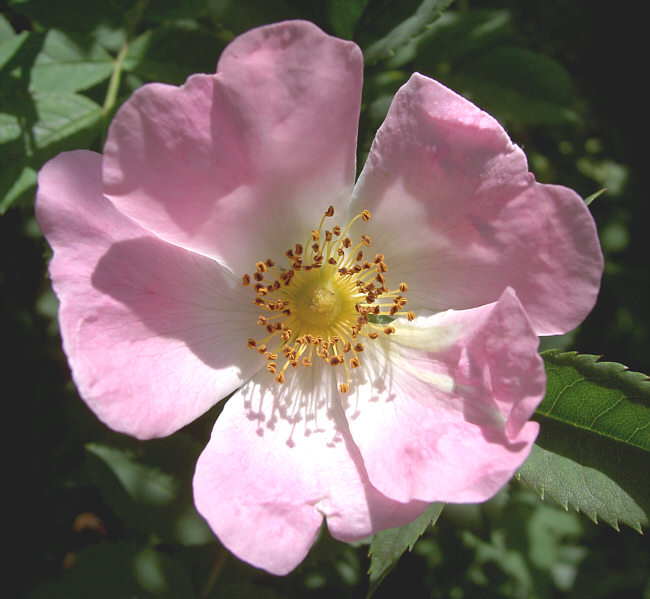
\includegraphics[width=0.3\textwidth]{Pic_DogRose.png}
 	\caption{Rosa canina (dog rose)~\cite{WikipediaDogRose}.}
 	\label{fig:DogRose}
\end{figure}

\begin{figure} 
 	\centering
 		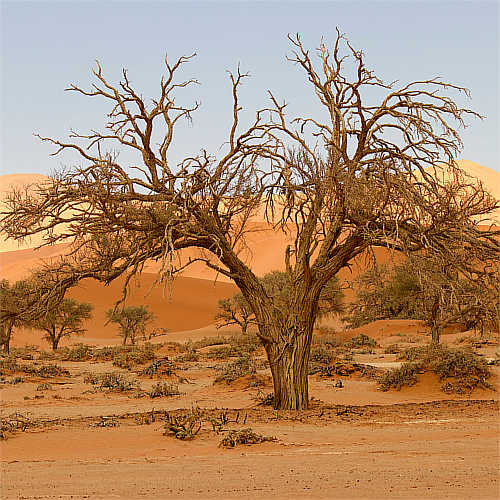
\includegraphics[width=0.3\textwidth]{Pic_Tree.png}
 	\caption{Biological tree branching structure~\cite{WikipediaTree}.}
 	\label{fig:IRLTree}
\end{figure}

\begin{figure} 
 	\centering
 		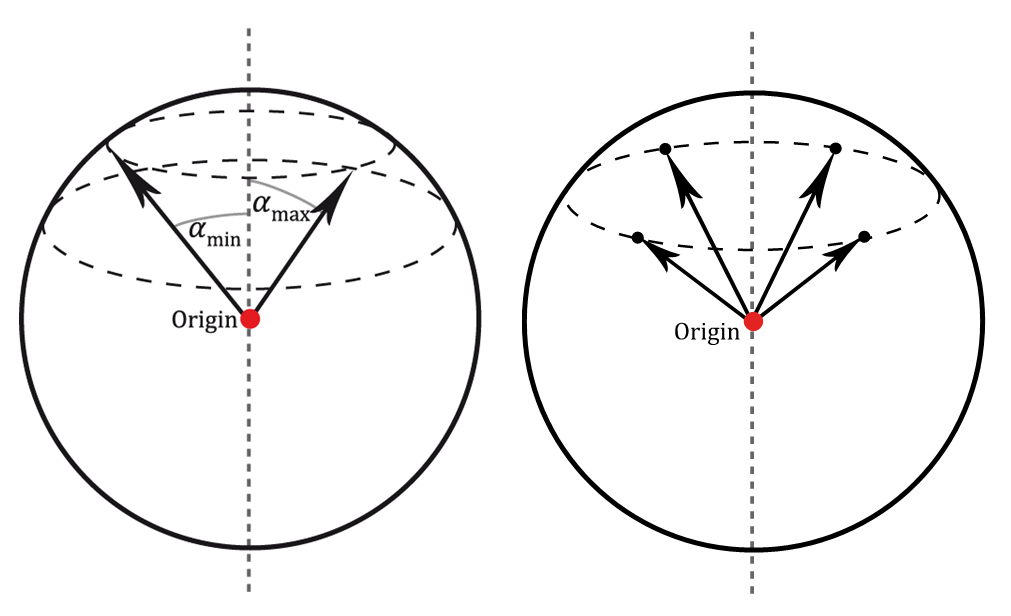
\includegraphics[width=0.6\textwidth]{Fig_SphereInOne.png}
 	\caption{Visualization of allowed freedom for a punctiform origin (left); even spread of four points with $\alpha_\text{min} = \alpha_\text{max}$ (right).}
 	\label{fig:FreedomSpheres}
\end{figure}

If we look at plant structures so different as rose blossoms (Figure~\ref{fig:DogRose}), dandelion seed heads or tree branching (Figure~\ref{fig:IRLTree}), it turns out that many of those follow a somewhat even spread, and the shapes of the various arrangements are describable by different degrees of freedom. In general, this freedom is radially symmetric in growth direction, so a full description may be given by two angles $\alpha_\text{min}$ and $\alpha_\text{max}$, defining the freedom of the distribution to deviate from the growth direction. The objects growing out of the origin then take positions such that the minimal distance between two objects is maximized---an even spread.

For punctiform origins, like those used in this project, the two angles define two circles on a sphere, and the directional possibilities are the set of vectors pointing from the origin to a point on the sphere between the two circles. Thus, a dandelion-like structure corresponds to a minimum deviation of $\alpha_\text{min} = 0$ (i.e., directions can be arbitrary close to the growth direction) and a maximum deviation of 
$\alpha_\text{max} \approx 90^\circ$. For ``flat'' layouts, like those of the petals of the rose in Figure~ \ref{fig:DogRose}, is $\alpha_\text{max} - \alpha_\text{min} \approx 0$ (or small, if there are different layers of petals).

If the number of objects that growth out of a given origin becomes small, such as in the tree in Figure~\ref{fig:IRLTree}, this principle is less obvious on first glance, but it remains a special case of $\alpha_\text{max} - \alpha_\text{min} \approx 0$. In the case of trees, the ``objects'' that growth out of the origins are actually branches, and can branch, i.e., form new origins, in itself. This is the self-similarity in the title of this chapter, and this is also the reason why L-systems can simulate tree-shapes so well, and why the golden ratio, being an expression of self-similarity, can be found in countless different contexts in biology.

The practical implementation of these principles obviously imposes difficulties, which were only solved by approximation in this project. For example, the distance of objects growing out of origins was approximated by the ``distance'' of growth directions only, and the algorithm used to generate these directions only yields semi-satisfactory results for $\alpha_\text{min} \neq \alpha_\text{max}$. More variety in basic forms was cut in scope in favor of factors of interacting growth---see Chapter~\ref{cptr:Influencing}.

\section{Implementation}
\subsection{Engine, Language and Code}
The implementation was done in Unreal Engine 4 (UE4 or UE in short)~\cite{WhatIsUnreal}, a framework developed by Epic Games. Originally meant to be used as a basis for video games, it soon found applications in many different fields after it became available to the general public in 2014. It offers a strong framework for efficient rendering, collision detection, physics and alike (i.e., it solves many fundamental but hard 3D problems) and is completely free of charge for use cases likes ours. Especially the collision detection systems were used extensively in this project, and UE's ample debugging and performance profiling tools proofed very helpful at various points in development, too. 

Most of the code was done in C++, as especially the generation of the organisms is very performance critical. Blueprints, the visual scripting language of Unreal, was only used occasionally for prototyping and non-heavy-lifting work, e.g., keyboard input handling and variable/property setup.

One major development obstacle was that each cell needs to be represented by a single mesh, imposing a problem, as Unreal usually can handle around 1200 draw calls per frame if 60~fps are supposed to be hit. Thus, UE projects can easily be CPU-bottlenecked, even though the amount of rendered polygons is not exhausting the capabilities of the graphics card. So, geometry instancing was used, in the form of Instanced Static Meshes~\cite{UEInstancing}, which is one of the UE variants of this practice. Instanced Static Meshes render the same 3D model multiple times per draw call, improving the rendering speed by several orders of magnitude. On the downside, the difference between instances is limited to scale, size and rotation, and the system is noticeably less flexible than Spline Meshes~\cite{UESplines}, which would commonly be used to represent linearly arranged meshes.

\subsection{Modelled Behaviors} \label{cptr:Influencing}
The following behaviors are simulated:
\begin{itemize}
	\item Plants in water are allowed to have more cells than those without access to it.
	\item Wind/storm blows over a part of the stage, destroying parts of plants that get hit by to much wind.
	\item There is a cone-shaped light source, leading plants to grow in the direction of the light as they divide faster on the light-faced site, have smaller leafs and to have a higher total cell count.
	\item The diameter of cells grows when a higher ``weight'' rest on them, i.e., when they have many attachment descendants.
	\item The growth direction can have a positive or negative correlation with gravity, leading to trees that always grow upward, and trees that ``bend over'', even off the stage.
	\item Cells divisions cannot result in children that collide with external objects or other cells of the plant. Figure~\ref{fig:SelfCollision} shows an example.
		\begin{figure} 
 		 \centering
 		    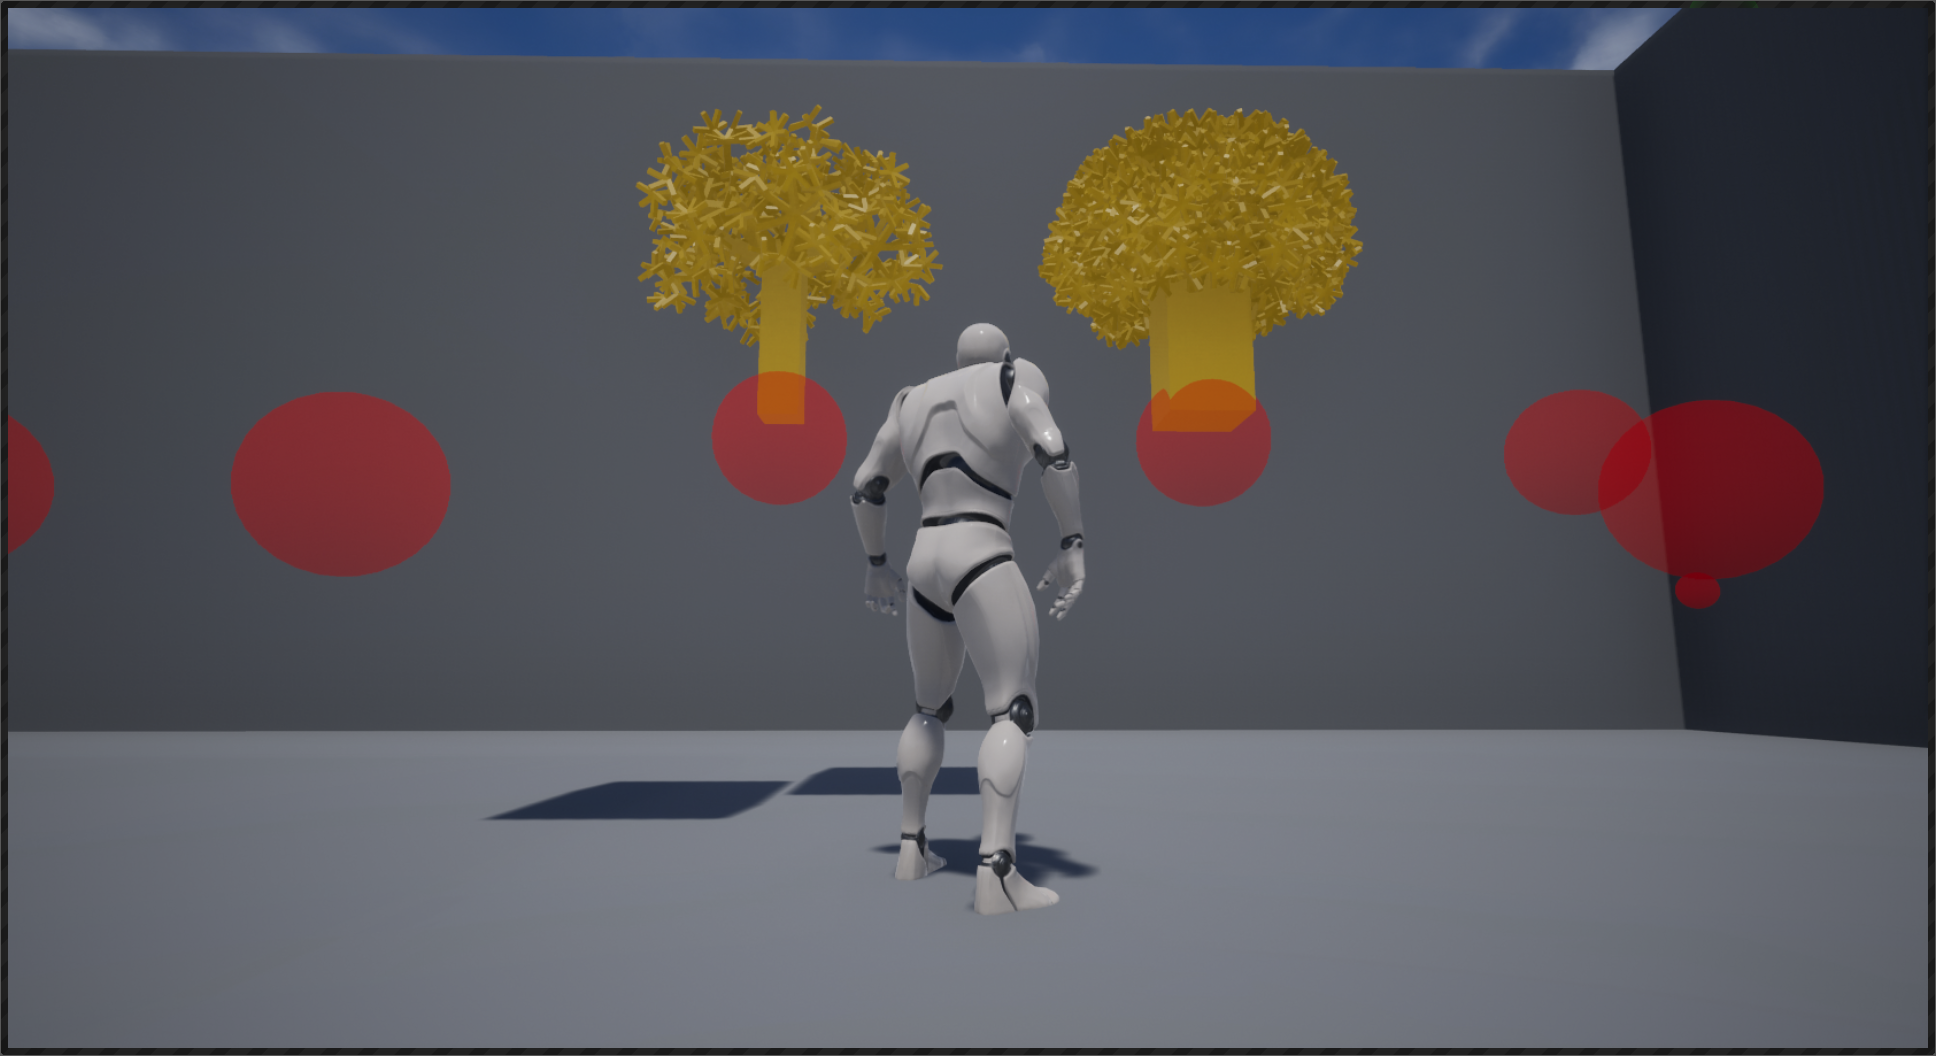
\includegraphics[width=0.6\textwidth]{SS_SelfCollision.png}
 		 \caption{Self collision enabled (left) and disabled (right).}
 		 \label{fig:SelfCollision}
	\end{figure}
	\item Certain cells---in this case the roots---can grow attached to the ground and up to walls when they hit them (Figure~\ref{fig:RootsOnFloor}).
	\begin{figure} 
 		 \centering
 		    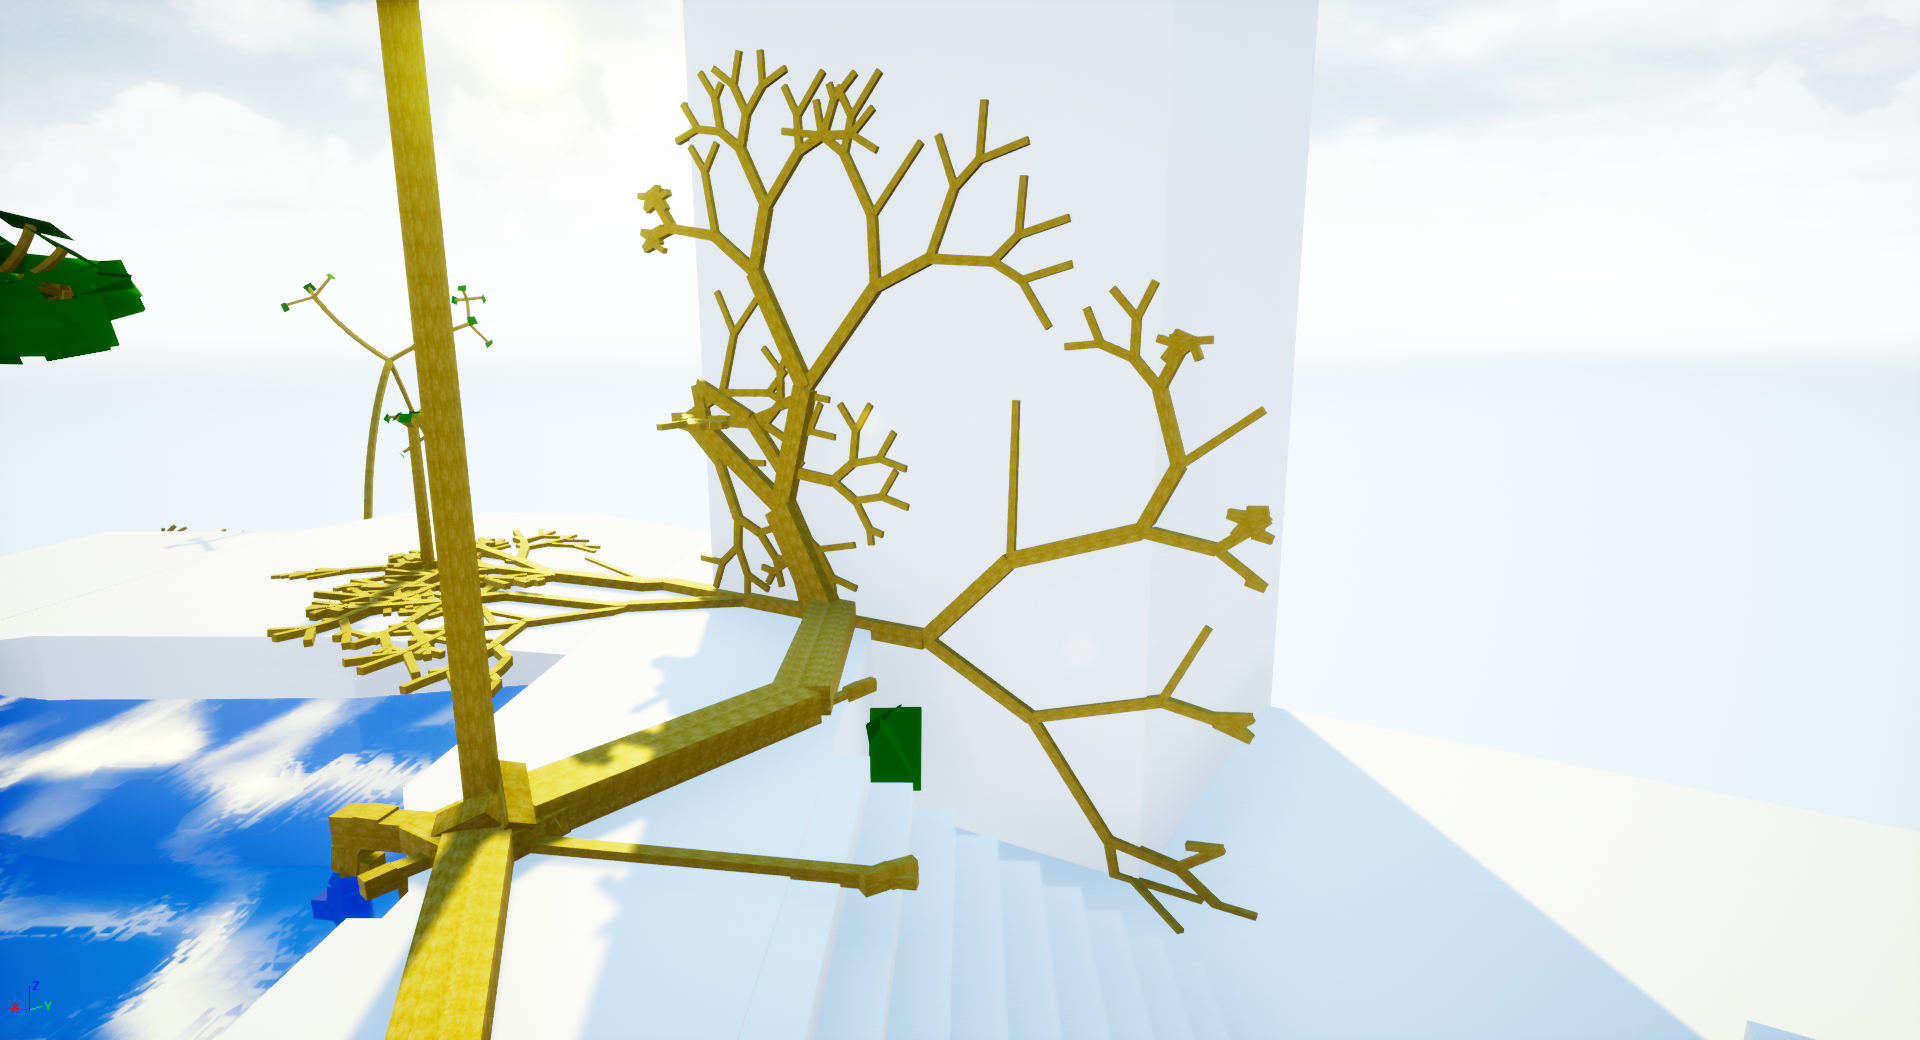
\includegraphics[width=0.6\textwidth]{SS_Roots.png}
 		 \caption{Roots growing on the floor and up a wall.}
 		 \label{fig:RootsOnFloor}
	\end{figure}
\end{itemize}
As hinted above, the numerous collision features of Unreal were used extensively. On the one hand directly to check for overlapping collision shapes (e.g., for the water mechanics) or in the form of ``Raycasts/Line Traces'' that determine where a point that travels on a given line segment hits something. This was, for example, used for the light and wind mechanics, which are modeled by around 10,000 Raycasts each growth iteration.
One possible influence of light is shown in Figure~\ref{fig:GrowToLight}. The light comes from the left, and the source is very close to the tree on the left. This tree has noticeably more leafs and children than the one further in the background, even though the genetics/properties of the plants are the same. Additionally, it can be clearly seen how the tree divided more on the site facing the light source. The image also shows nicely the vastly different possible diameters of cells depending on the number of attachment descendants they have, and the effect of the trees bending upwards as they have a positive correlation with gravity. 

\begin{figure}
 	 \centering
 	    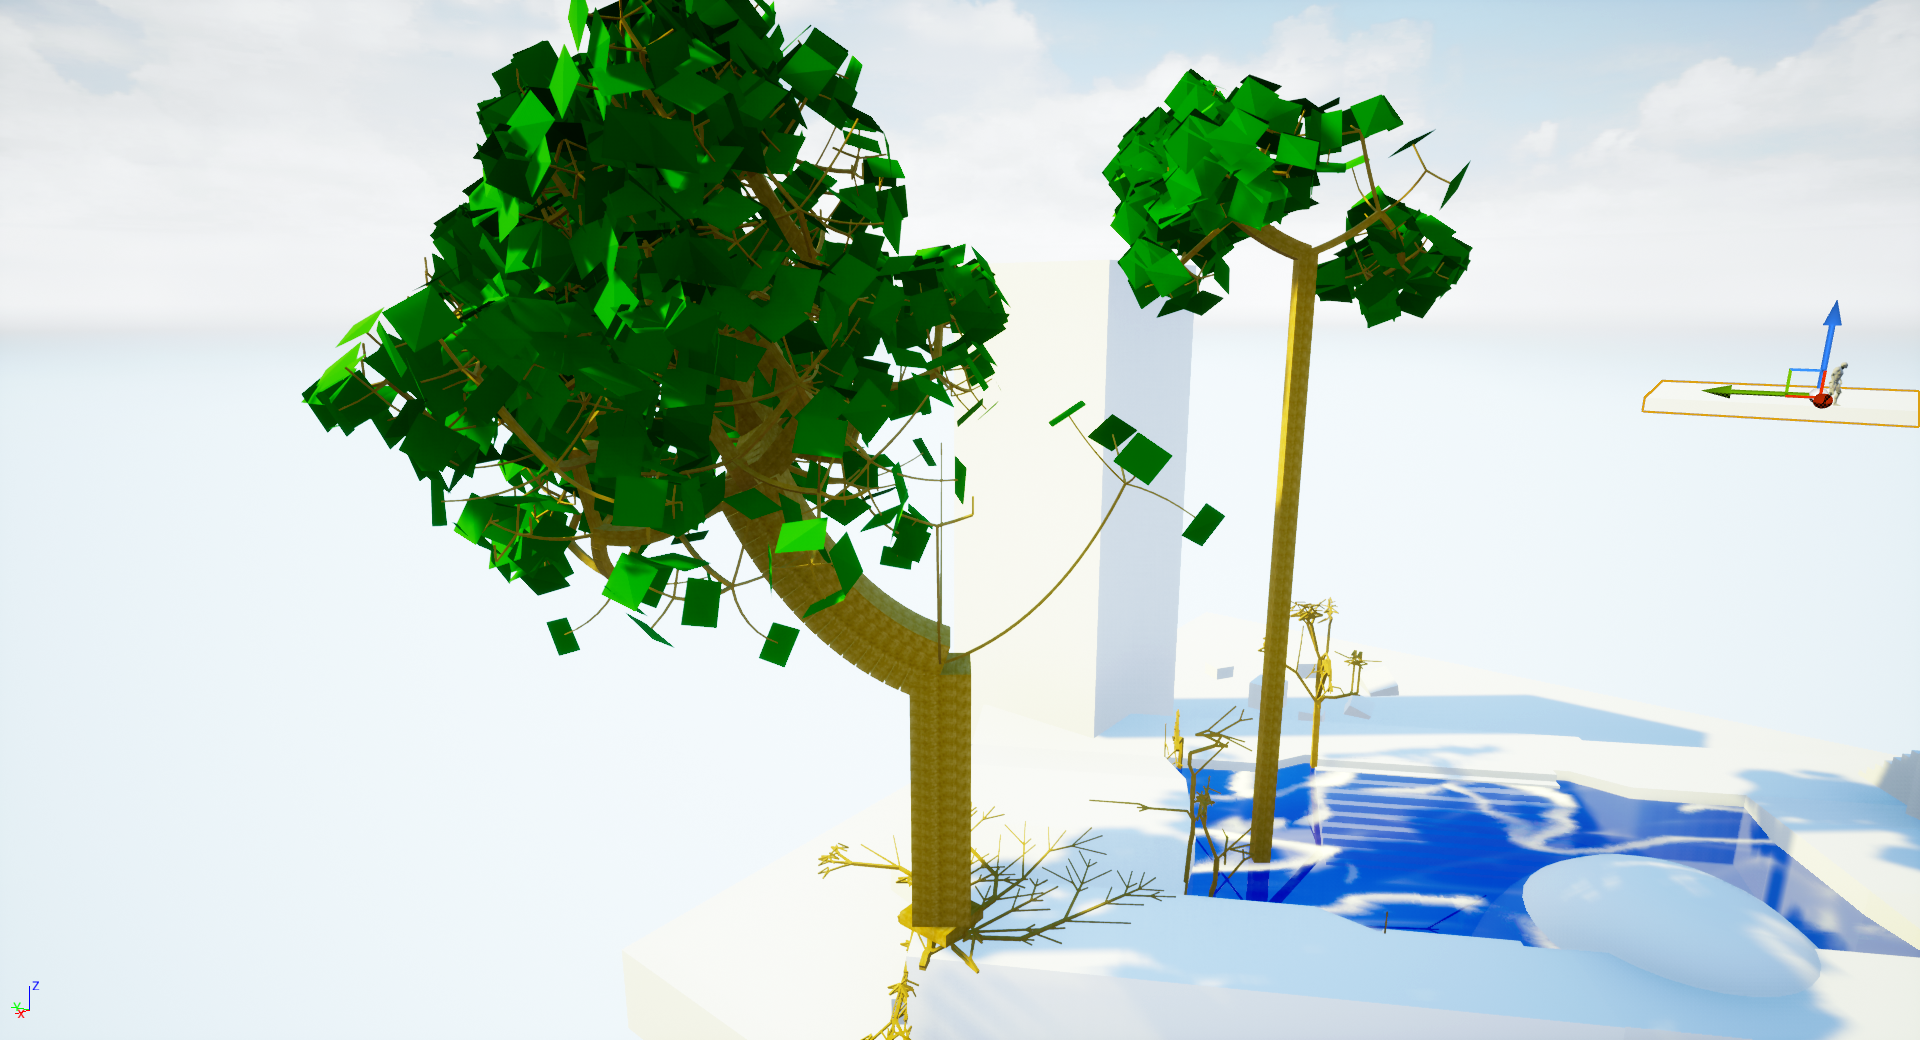
\includegraphics[width=0.6\textwidth]{SS_GrowToLight.png}
 	 \caption{Influence of different light conditions on plants with identical genetics.}
 	 \label{fig:GrowToLight}
\end{figure}

\subsection{Paramteter / Division Rules}
In its very fundamentals, the used division schemes are based on three states, $K$, $F$ and $H$ ($A \rightarrow B$ means that $A$ divides into $B$):

\begin{align}
	&K \xrightarrow {\text{time}}, F, H \quad \text{(vertical)} \label{eq:K} \\
	&F \xrightarrow {\text{time}}, F, F \quad \text{(vertical)} \label{eq:F}\\
	&H \xrightarrow {\text{light}}, \overbrace{ K, \ldots , K}^{k} \quad \text{(horizontal)}  \label{eq:HLight} \\
	&H \xrightarrow {\text{time}}, \overbrace{ K, \ldots , K}^{k'} \quad \text{(horizontal)} \label{eq:HTime}
\end{align}

``Vertical'' division means that resulting cells are aligned such that every cell has one attachment child, and one attachment parent (i.e., the growth is ``straight''). ``Horizontal'' division means that all new cells have the same parent as the initial cell, and are spread evenly according to Chapter~\ref{cpt:EvenSelfSim}.

For the branches, the cells with state $H$ are the leafs, and in these sense Equation~(\ref{eq:HLight}) defines the way a leaf divides if a certain amount of light hits it in a given iteration. Equation~(\ref{eq:HTime}) defines leaf division independent of light. In general is $k > k'$, to establish the behavior of trees growing towards light, in the sense that they divide more into this direction. Roots follow the same scheme, with different settings though, and their even spread is only in a plane and not full 3D space.

Regarding Equation~(\ref{eq:F}), there are actually multiple $F$ states, to allow a slowing down of branch growth (i.e., cells that divided out of a $H$ in very recent iterations have a faster division rate than ``older'' ones). In Equation~(\ref{eq:K}), the time is one iteration, while it is a plant property in Equations (\ref{eq:F}) and (\ref{eq:HTime}).

\subsection{Packaged Project and Controls}
The compile of the project is constituted of two parts: One map where it is possible to set values (e.g., leaf size) for a given tree at runtime and see the distinct possible results, and one map that generates and randomizes many multiple plants, i.e., a ``forest''.

Switching from one map to the other is done by pressing \texttt{M} on the keyboard. The control of the character (``Mannequin'') is the same for both maps: jumping and flying is done by pressing \texttt{Space}, and the movement itself is done via industry-standard \texttt{WASD}/mouse controls. \texttt{P} toggles the rendering of leafs. \texttt{I} updates the tree from the input values on the value manipulation map and adds ten rendering iterations on the forest map. \texttt{O} rerandomizes the values of the single tree, and resets the whole forest on the respective maps.


\section{Results}
\subsection{Complex Interactions}

For closeness to reality and performance reasons, the number of cells per organism needs to be limited. When simulating multiple or many trees at once, we used this constraint as an additional basis for interaction between organisms and their environment: If tree leafs get hit by light, or tree cells overlap with water, the total amount of cells allowed in the corresponding organism is increased. The influence of light on allowed cell count can be clearly seen in the already mentioned Figure~\ref{fig:GrowToLight}, and without the influence of water on the tree in the back, the differences would be even more notable.

\begin{figure}
 	 \centering
 	    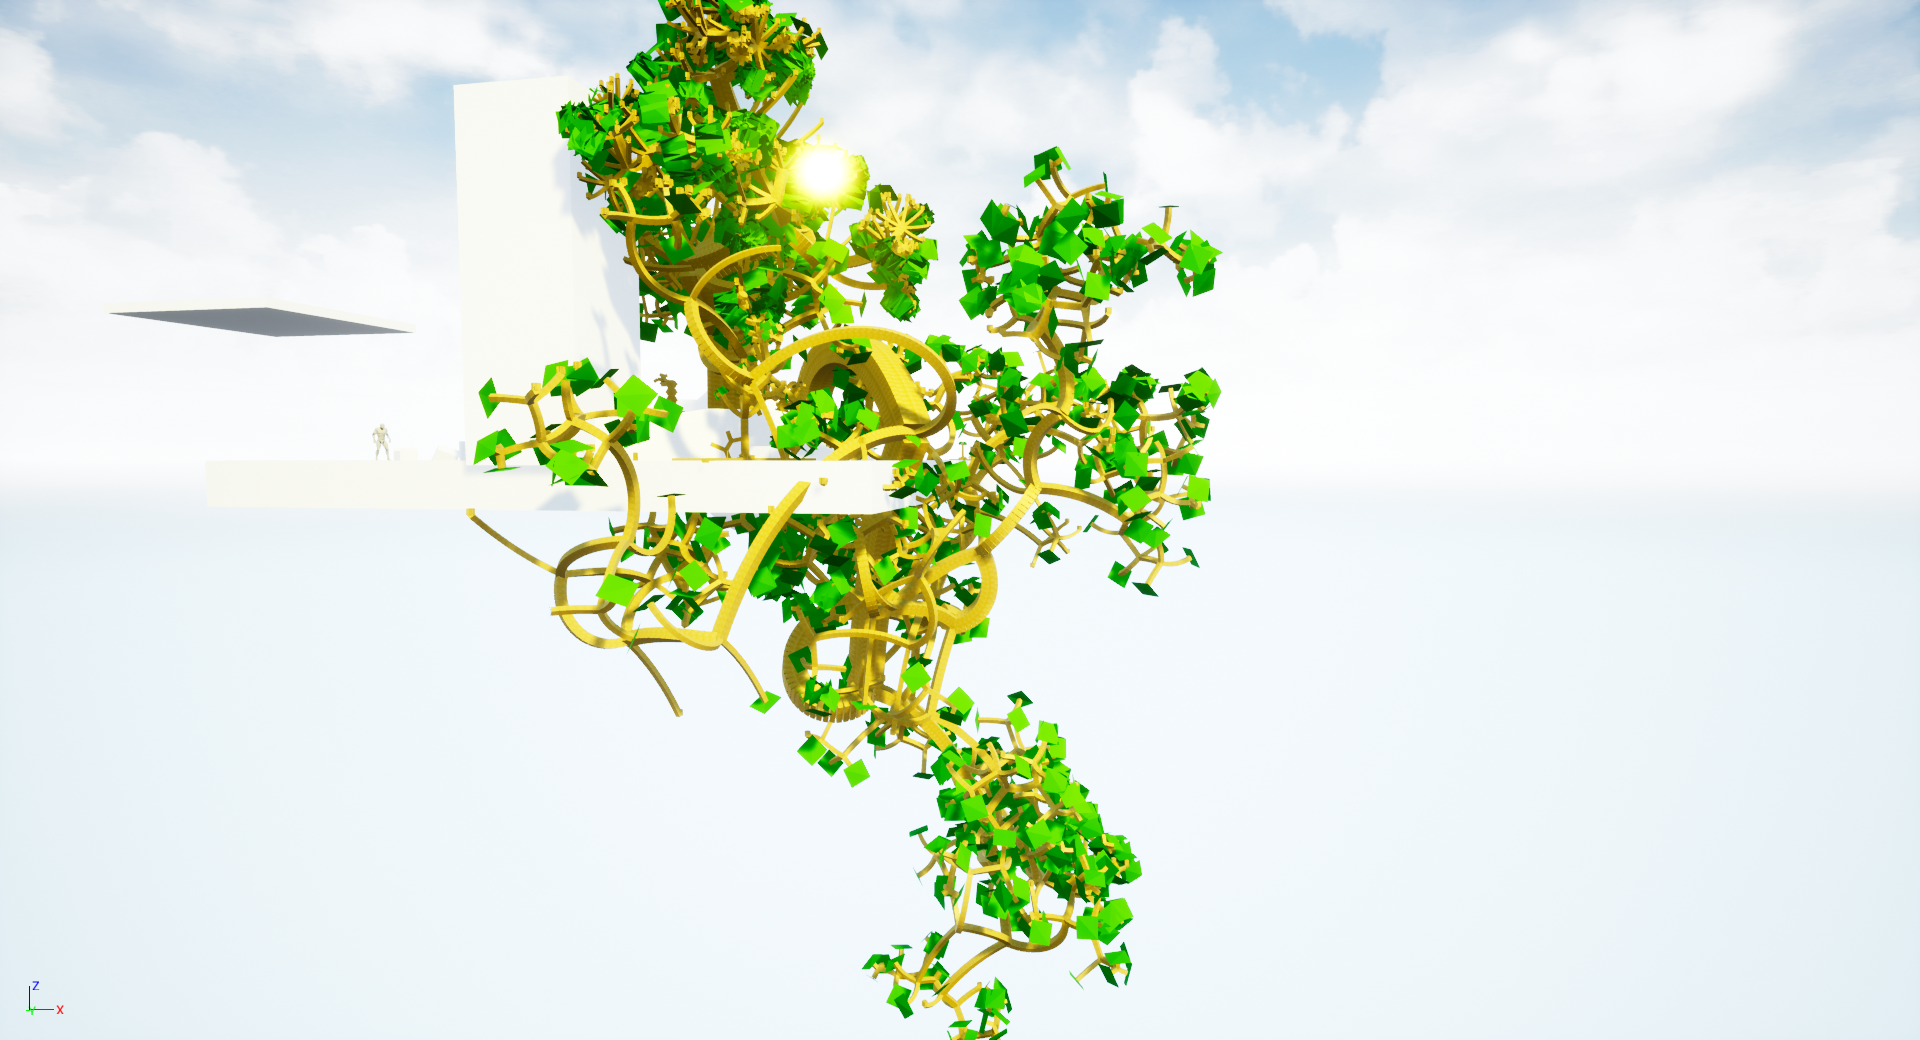
\includegraphics[width=0.6\textwidth]{SS_BIGTree.png}
 	 \caption{Massive tree taken out of an earlier version.}
 	 \label{fig:BIGTree}
\end{figure}

On the forest map, new trees appear where light hits the ground with randomized properties. Before, trees were spawned on random locations on the ground. As the light source is very close to the stage, this leads to the algorithm terminating after a few hundred iterations. This change also had one complex interaction we did not see coming beforehand: Very big trees, like the one seen in Figure~\ref{fig:BIGTree}, seem to be impossible or at least very improbable now. As far as we can see, these trees occurred if a plant got spawned in the water with a negative correlation with gravity such that the tree bended towards the light, getting both bonuses at once. This is not possible to this extent otherwise, as the water on the stage is a small distance away from the light source. Now, the spawn positions in the water closest to the light are no longer possible, as the rim of the water basin blocks the light Raycast to these spawn locations. Even though this connection was not examined super thoroughly, it definitely resembles an intriguing interaction.

\begin{figure}
 	 \centering
 	    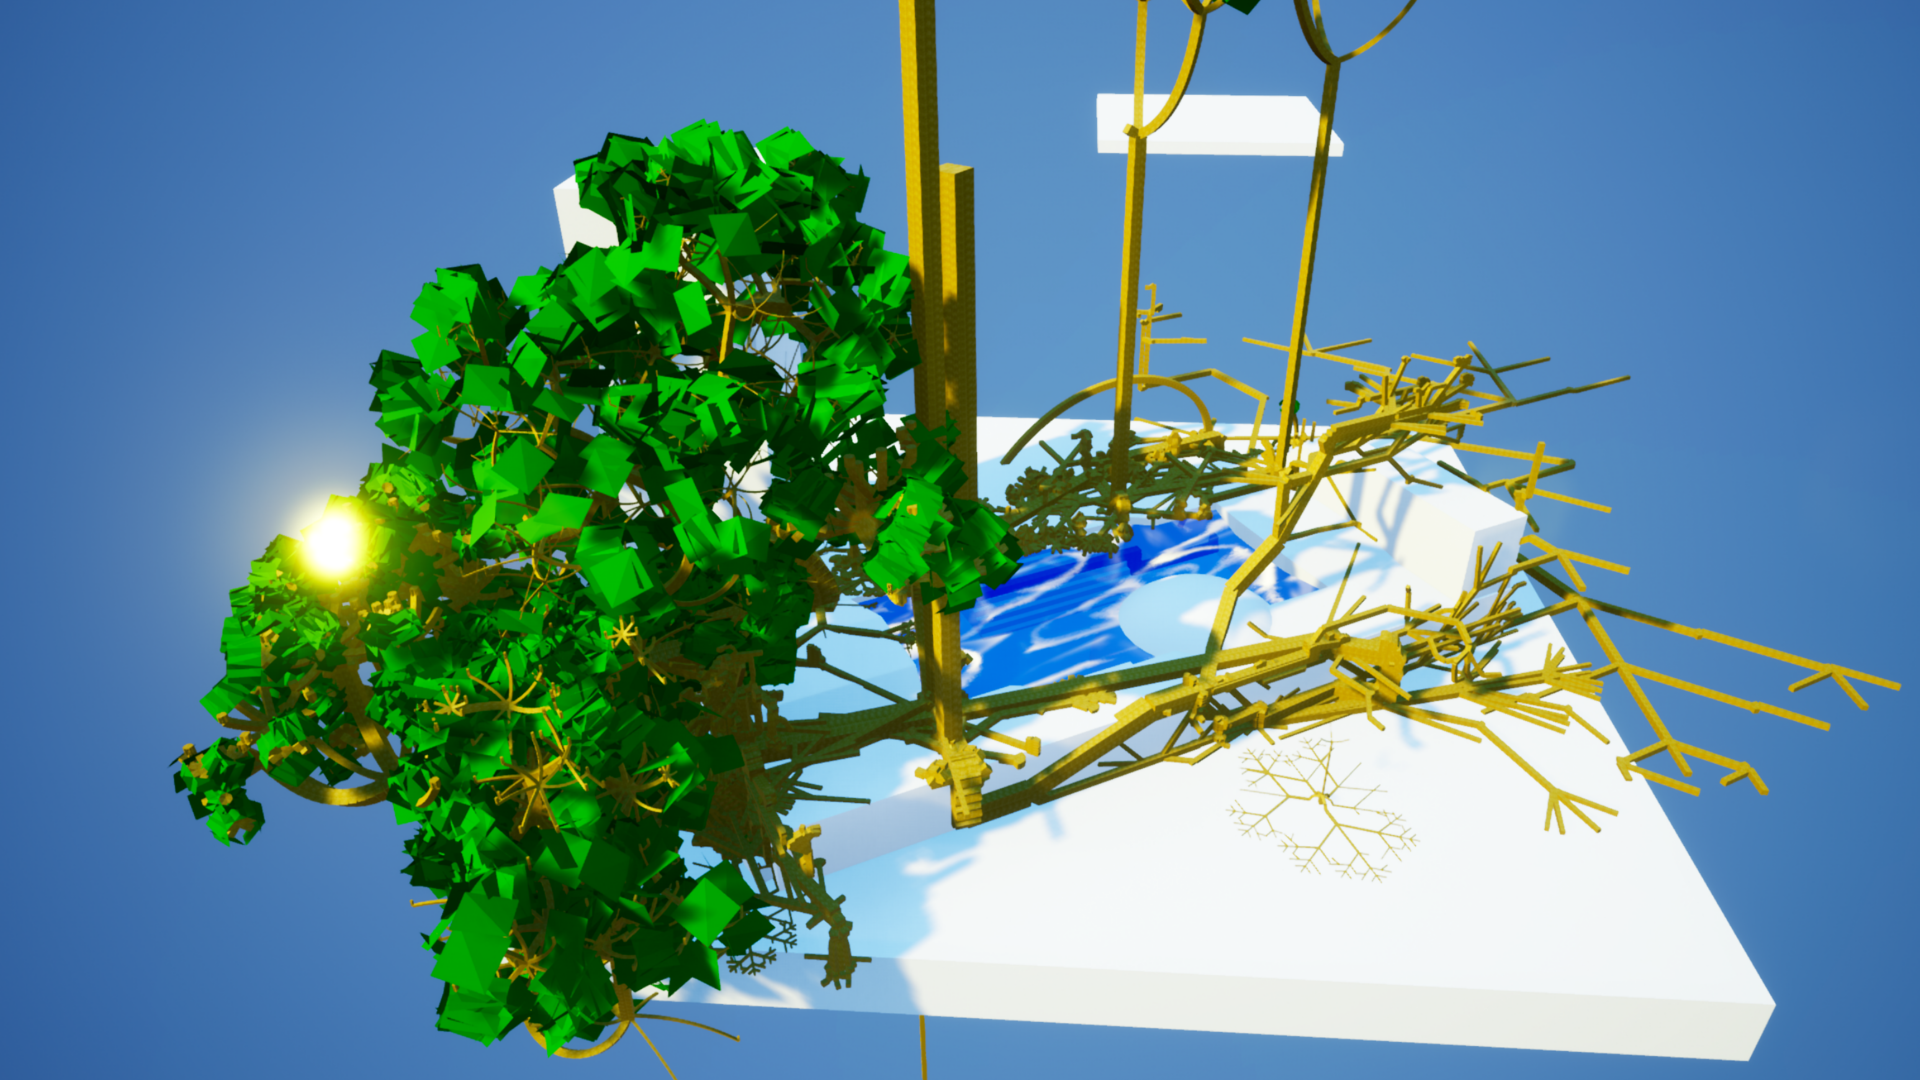
\includegraphics[width=0.6\textwidth]{SS_StageWithWind.png}
 	 \caption{Terminated algorithm with visible influences of wind.}
 	 \label{fig:StageWind}
\end{figure}

\begin{figure}
 	 \centering
 	    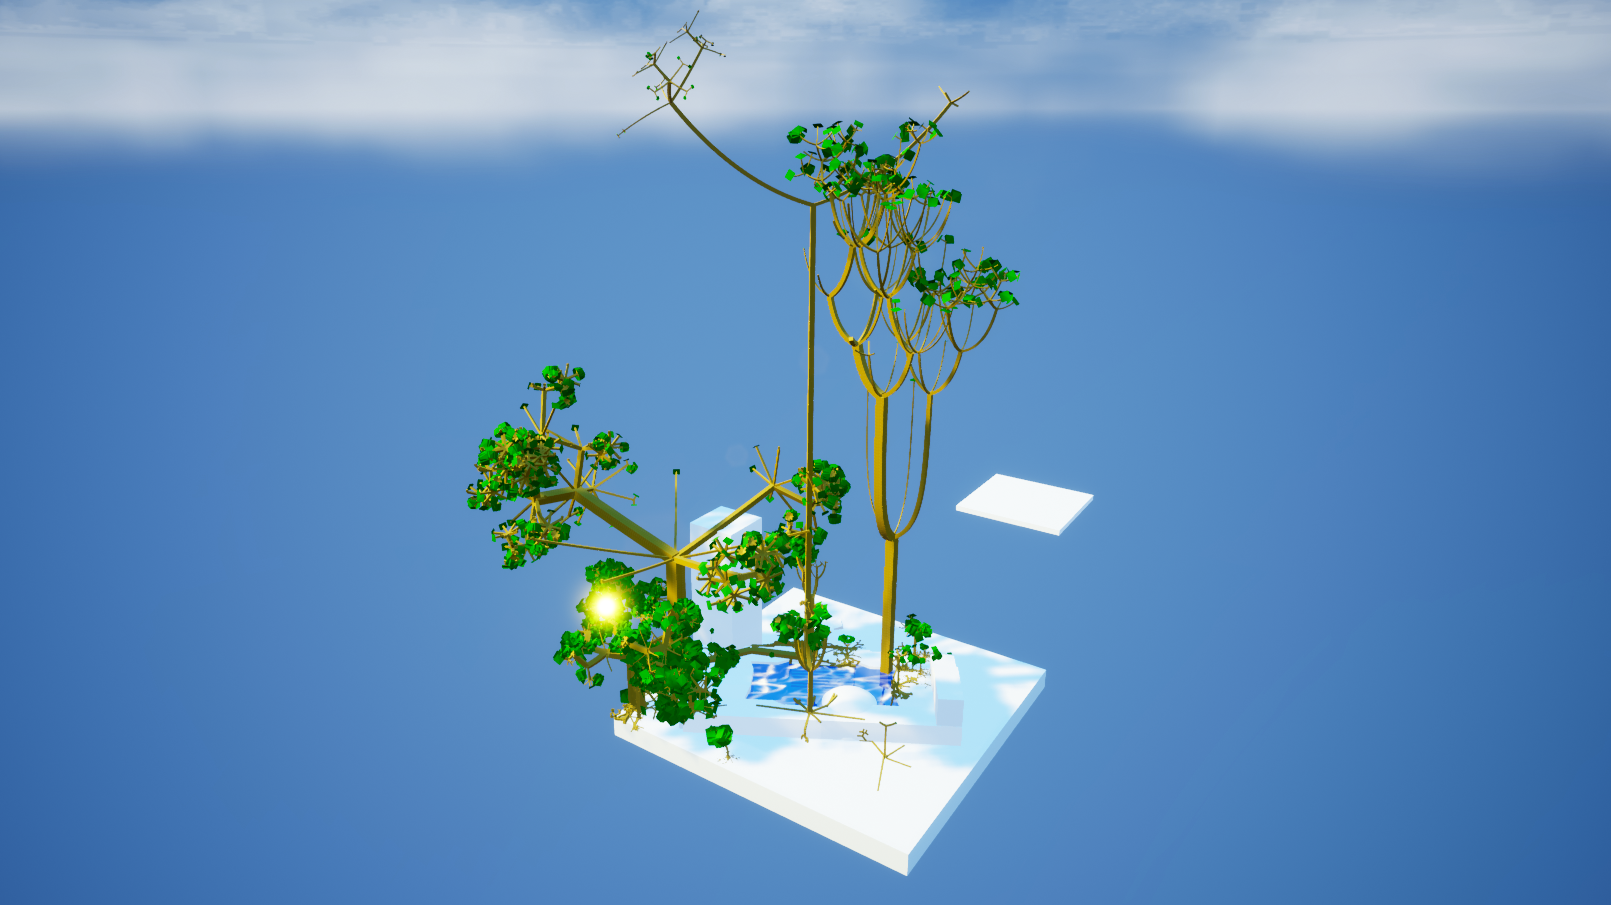
\includegraphics[width=0.6\textwidth]{SS_StageTallTrees.png}
 	 \caption{Difference of tree shape in water and near to light (reduced wind).}
 	 \label{fig:StageTallTrees}
\end{figure}

Figure~\ref{fig:BIGTree} also shows the limits of the collision detection system: As it is only activated on leafs and trunks without attachment children, division of cells closer to the root might break the system. Especially plants bending with gravity show this behavior and grow through the stage's floor. Figure~\ref{fig:StageWind} and Figure~\ref{fig:StageTallTrees} show two possible states after the algorithm terminated. Right in the center of Figure~\ref{fig:StageWind} one is also able to see cut off trunks and branches: those are in the corridor of the wind and did not have the stability to resist it. Figure~\ref{fig:StageTallTrees} on the other hand shows another interesting result: the different growth patterns of trees in the water and trees near the light source. The latter do not divide their leaves as often, thus the relevance of their trunks growth is more dominant, leading to trees growing into the sky rather than increasing width. There are way more extreme examples, but those are obviously even more cumbersome to depict.

All in all, the shown results are definitely a positive indication that the desired complex and surprising behavior is possible on the basis of the developed system.

\subsection{Performance}
When no tree growth iteration is calculated, the program hits constant 60~fps in all circumstances on the used Nvidia GTX~760 and Intel i5-4670K~3.40GHz. On the other hand, the performance of the iteration algorithm itself is hard to specify, as the positioning and properties of the iterated trees lead to vastly different behaviors and thus needed calculations. In the table below, two snapshots from different runs on the forest map are given for the time needed for different tasks in a single iteration cycle.
\begin{center}
\begin{tabular}{ | l | l l |}
\hline
	& Run $A$ & Run $B$\\
\cline{2-3}
  Meshes Calculation \& Setup  & 109.137 ms & 17.924 ms\\
  Cell Division in Data Structure & 51.654 ms & 4.699 ms\\
  Raytrace for Light & 19.551 ms & 15.450 ms\\
  Raytrace for Wind & 8.910 ms & 9.611 ms \\
  Weight \& Wind Burden & 2.146 ms & 4.769 ms\\
  Water Influence & 0.016 ms & 1.064 ms\\
  Total Iteration Time & 191.473 ms & 53.595 ms\\
\hline
\end{tabular}
\end{center}

This times were measured in the ``Play in Editor'' feature of the Unreal Engine, and compiled programs are substantially faster. Nevertheless, these snapshots may provide an overview of the proportions of the calculation times, even though they can vastly differ: The time solely needed for low level cell division is more than 10 times bigger in $A$ than in $B$, and the total execution time differs by a factor of nearly 4. It should also be added that the representativity of the two measurements needs to be taken with a grain of salt, especially for the water interaction calculation time.

\section{Conclusion}
In this work, we presented an approach to abstract plant growth in a non-standard way, based on even spreads, self-similarity, and influencing ecological factors. From our perspective, there seem to be two possible directions that seem interesting to improve on: On the one hand, the built system resembles a basis to simulate whole ecosystems in an interactable manner, and could be extended to include some form of nutrient circulation. For example, organisms could take some sort of resource from the ground for growth, which then cannot be used by others plants. The resource would be returned to the ground by tree dead (by age, illness or similar simulated causes) and decomposers that feed on the leftovers of other organisms and recycle the nutrients for the ecosystem. Later, even completely differently constructed organisms could be added to the system, i.e., ``animals'' that move around the stage and consume parts of plants.

On the other hand, the range of possibilities describable in the terms of Chapter~\ref{cpt:EvenSelfSim} could really only be scratched at the surface. So, another natural way to expand the project / research would be to try to recreate other plantal features with the developed algorithms by different divide properties, or to improve on those algorithms to yield more satisfying results (especially for $\alpha_\text{max} - \alpha_\text{min}$ big). The same holds for taking actual shapes into account when calculating even splits, and extensions to allow non-punctiform origins (e.g., for pine cone shaped growth behavior).

In these two directions, countless different features might be added. Maybe it even seems as this work is merely a starting point, and the extended applications definitely seem very interesting---be it in a more close to reality simulation-oriented context, or as an element of an actual game.

\begin{thebibliography}{99}
	\bibitem{MinecraftTree}  \href{https://minecraft.gamepedia.com/Tree}{Minecraft Wiki: ``Tree', minecraft.gamepedia.com/Tree}, viewed on 01/13/19
	\bibitem{Spore}  \href{https://en.wikipedia.org/wiki/Spore_(2008_video_game)}{Wikipedia: ``Spore'', en.wikipedia.org/wiki/Spore\_(2008\_video\_game)}, viewed on 01/13/19
	\bibitem{CellLab}  \href{http://cell-lab.net/}{Cell Lab website, cell-lab.net/}, viewed on 01/13/19
	\bibitem{EcoGame}  \href{https://www.strangeloopgames.com/eco/}{Eco website, strangeloopgames.com/eco/}, viewed on 01/13/19
	\bibitem{SpeedTree}  \href{https://store.speedtree.com/}{SpeedTree website, store.speedtree.com/}, viewed on 01/13/19
	\bibitem{ClimbingPlants}  \href{http://www.cse.chalmers.se/~uffe/xjobb/climbingplants.pdf}{Johan Knutzen, ``Generating Climbing Plants Using L-Systems''}, viewed on 01/13/19
	\bibitem{WikipediaDogRose}  \href{https://commons.wikimedia.org/wiki/File:Hundsrose.jpg}{Wikimedia: ``Hundsrose.jpg'', commons.wikimedia.org/wiki/File:Hundsrose.jpg}, viewed on 01/13/19
	\bibitem{WikipediaTree} \href{https://commons.wikimedia.org/wiki/File:Baum_im_Sossusvlei.jpg}
	{Wikimedia: ``Baum im Sossusvlei.jpg'', commons.wikimedia.org/wiki/File:Baum\_ im\_Sossusvlei.jpg}, viewed on 01/13/19
	\bibitem{WhatIsUnreal}  \href{https://www.unrealengine.com/en-US/what-is-unreal-engine-4}{``Make Something Unreal'', unrealengine.com/en-US/what-is-unreal-engine-4}, viewed on 01/13/19
	\bibitem{UEInstancing}  \href{https://api.unrealengine.com/INT/API/Runtime/Engine/Components/UInstancedStaticMeshComponent/index.html}{UE API Documentation (api.unrealengine.com/): ``UInstancedStaticMeshComponent''}, viewed on 01/13/19
	\bibitem{UESplines}  \href{https://docs.unrealengine.com/en-us/Engine/BlueprintSplines/Overview}{UE Documentation (docs.unrealengine.com/en-us/): ``Blueprint Spline Components Overview''}, viewed on 01/13/19
	
\end{thebibliography}
\end{document}

